\subsection{Université de Laval}

A continuación presentamos los gráficos resultantes de realizar una \textit{traceroute} a la página de la Université de Laval\footnote{www2.ulaval.ca.}.

\begin{figure}[H]
    \centering
    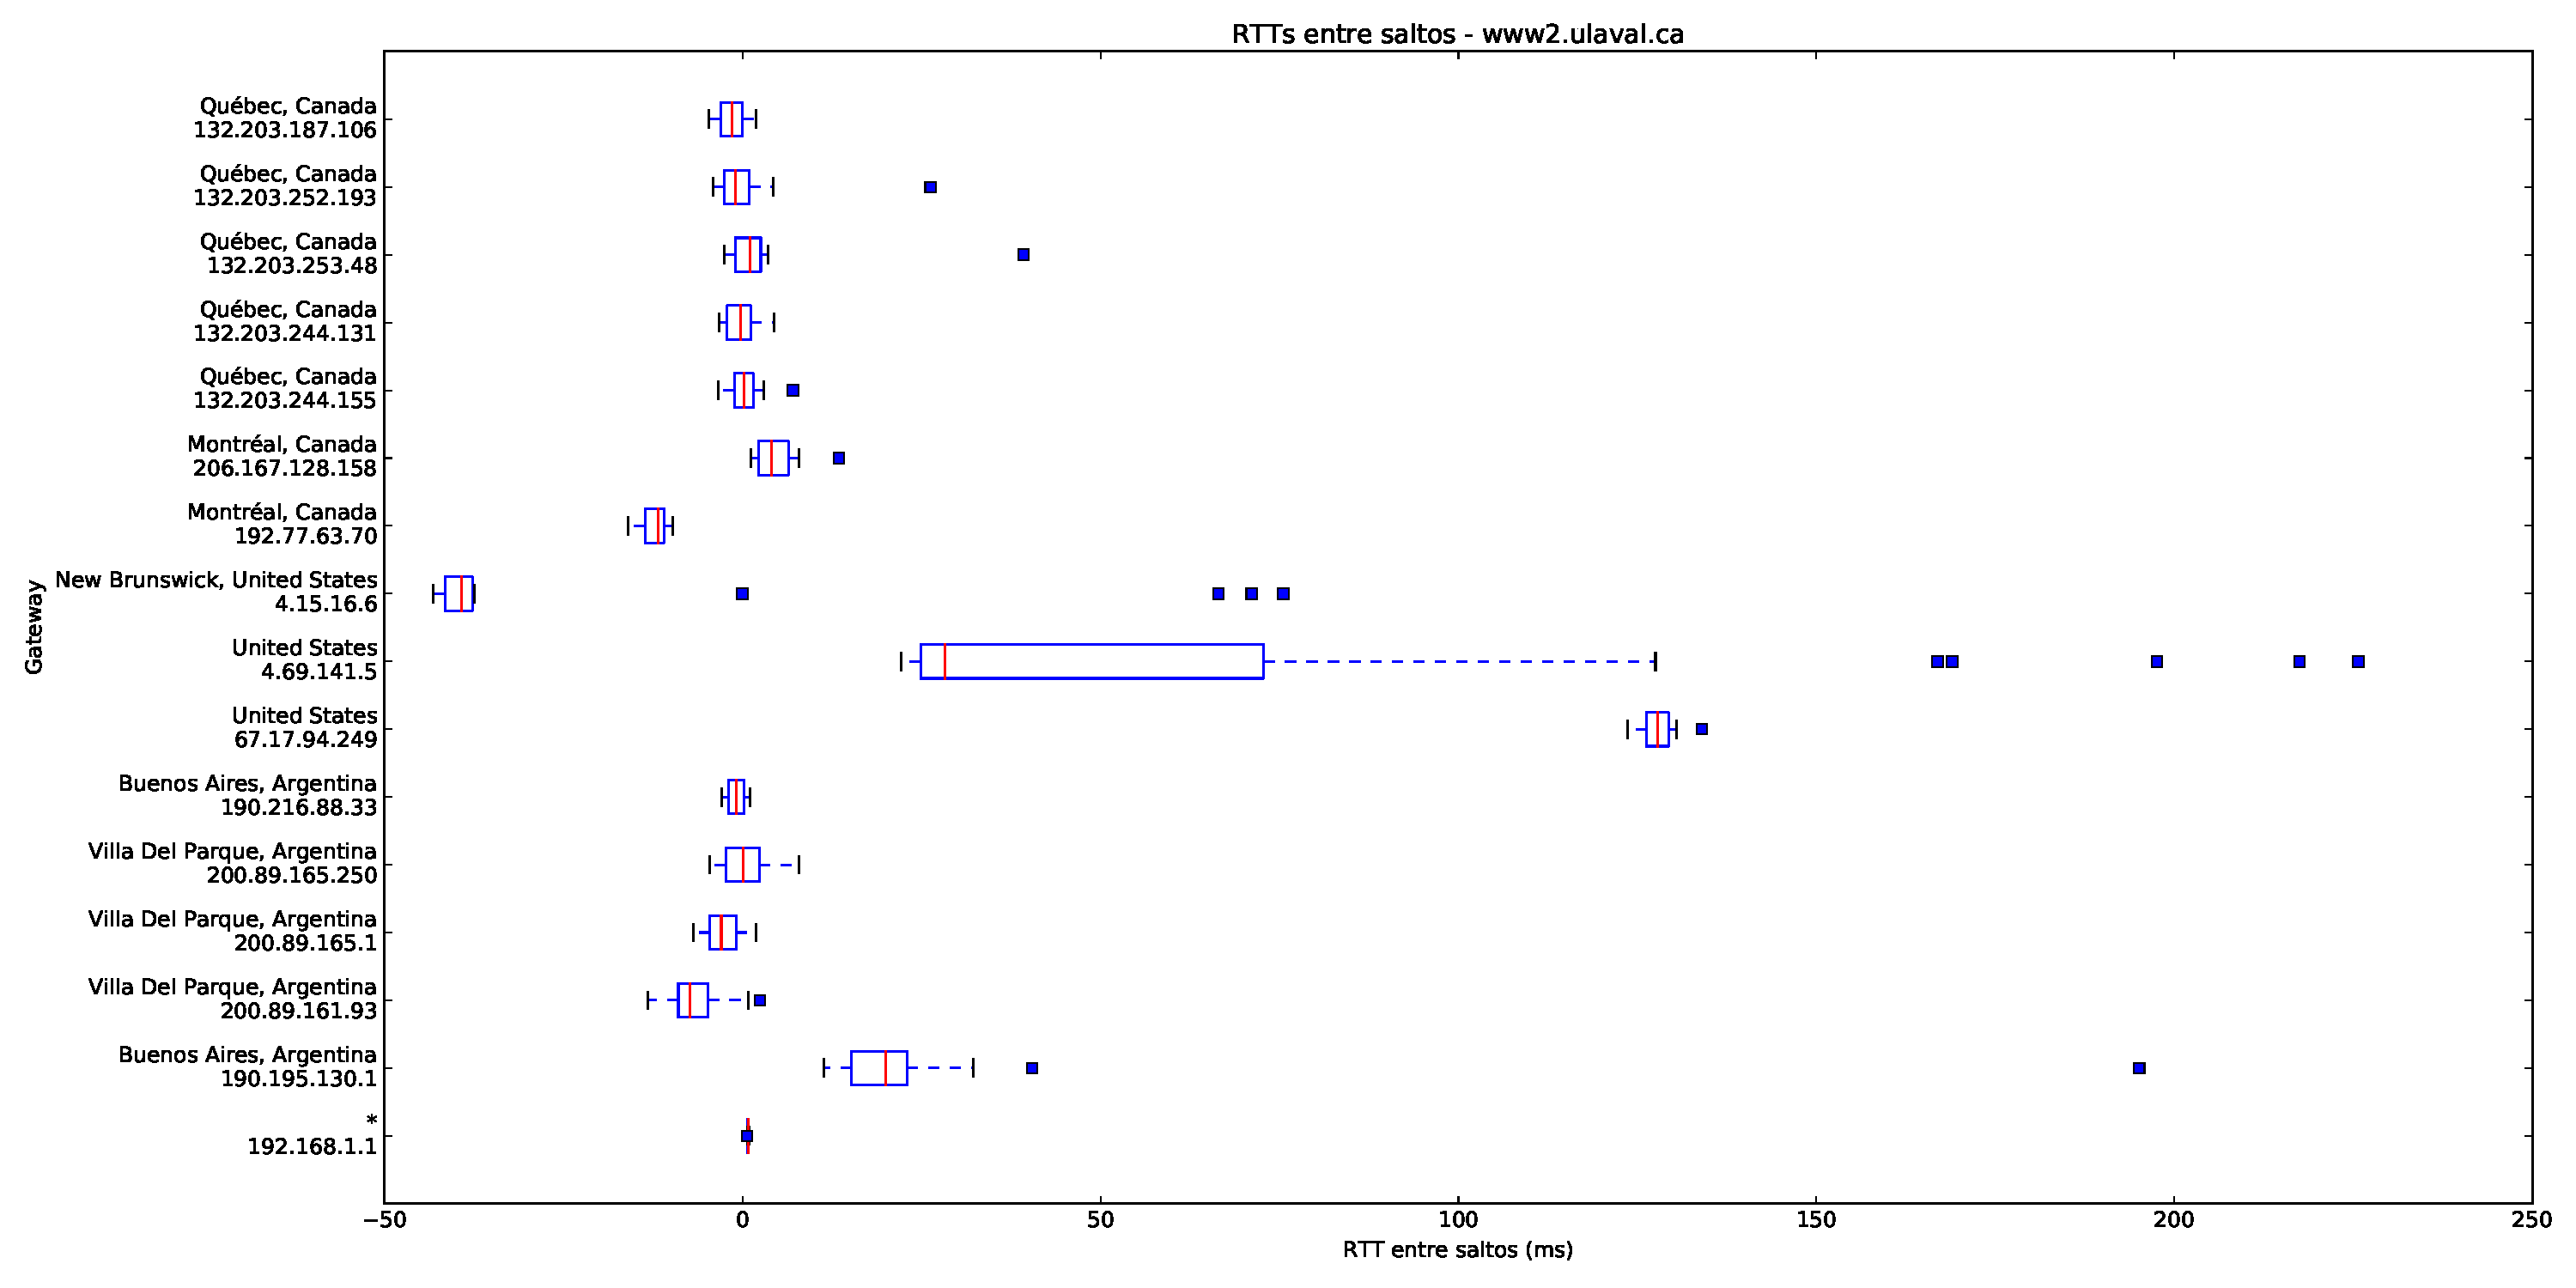
\includegraphics[width=8.5cm]{img/grafico1-www2-ulaval-ca.pdf}
    \caption{\normalfont RTTs entre saltos. El valor asignado al $i$-ésimo nodo corresponde al salto entre el $i$-ésimo y el $i - 1$-ésimo nodo. Para el primer nodo se utiliza simplemente su RTT.}
    \label{graf1L}
\end{figure}

\par En la realización de la \textit{traceroute}, 6 de los 22 ($27.\overline{27}\%$) nodos no respondieron los \textit{Time exceeded}.

\par Observamos una cantidad de \textit{outliers} y una desviación consistente entre los distintos saltos en la figura \ref{graf1L}.
Esto posiblemente se debe a una congestión momentárea en la red durante ciertas repticiones de la \textit{traceroute}, resultanto en que todos los RTTs de la repetición sean considerados \textit{outliers}.

\par Si bien la mayoría de los nodos presentan desviaciones similares, en el de dirección 4.69.141.5 se observa una varianza excepcionalmente alta.
Esto se puede deber a algunos de los factores mencionados en Jobst 2012\cite{anomalias}: métodos de balanceo de carga variando las rutas de los paquetes de diversas mediciones, o caminos de ida/vuelta asimétricos resultando en RTTs inconsistentes.

\begin{figure}[H]
    \centering
    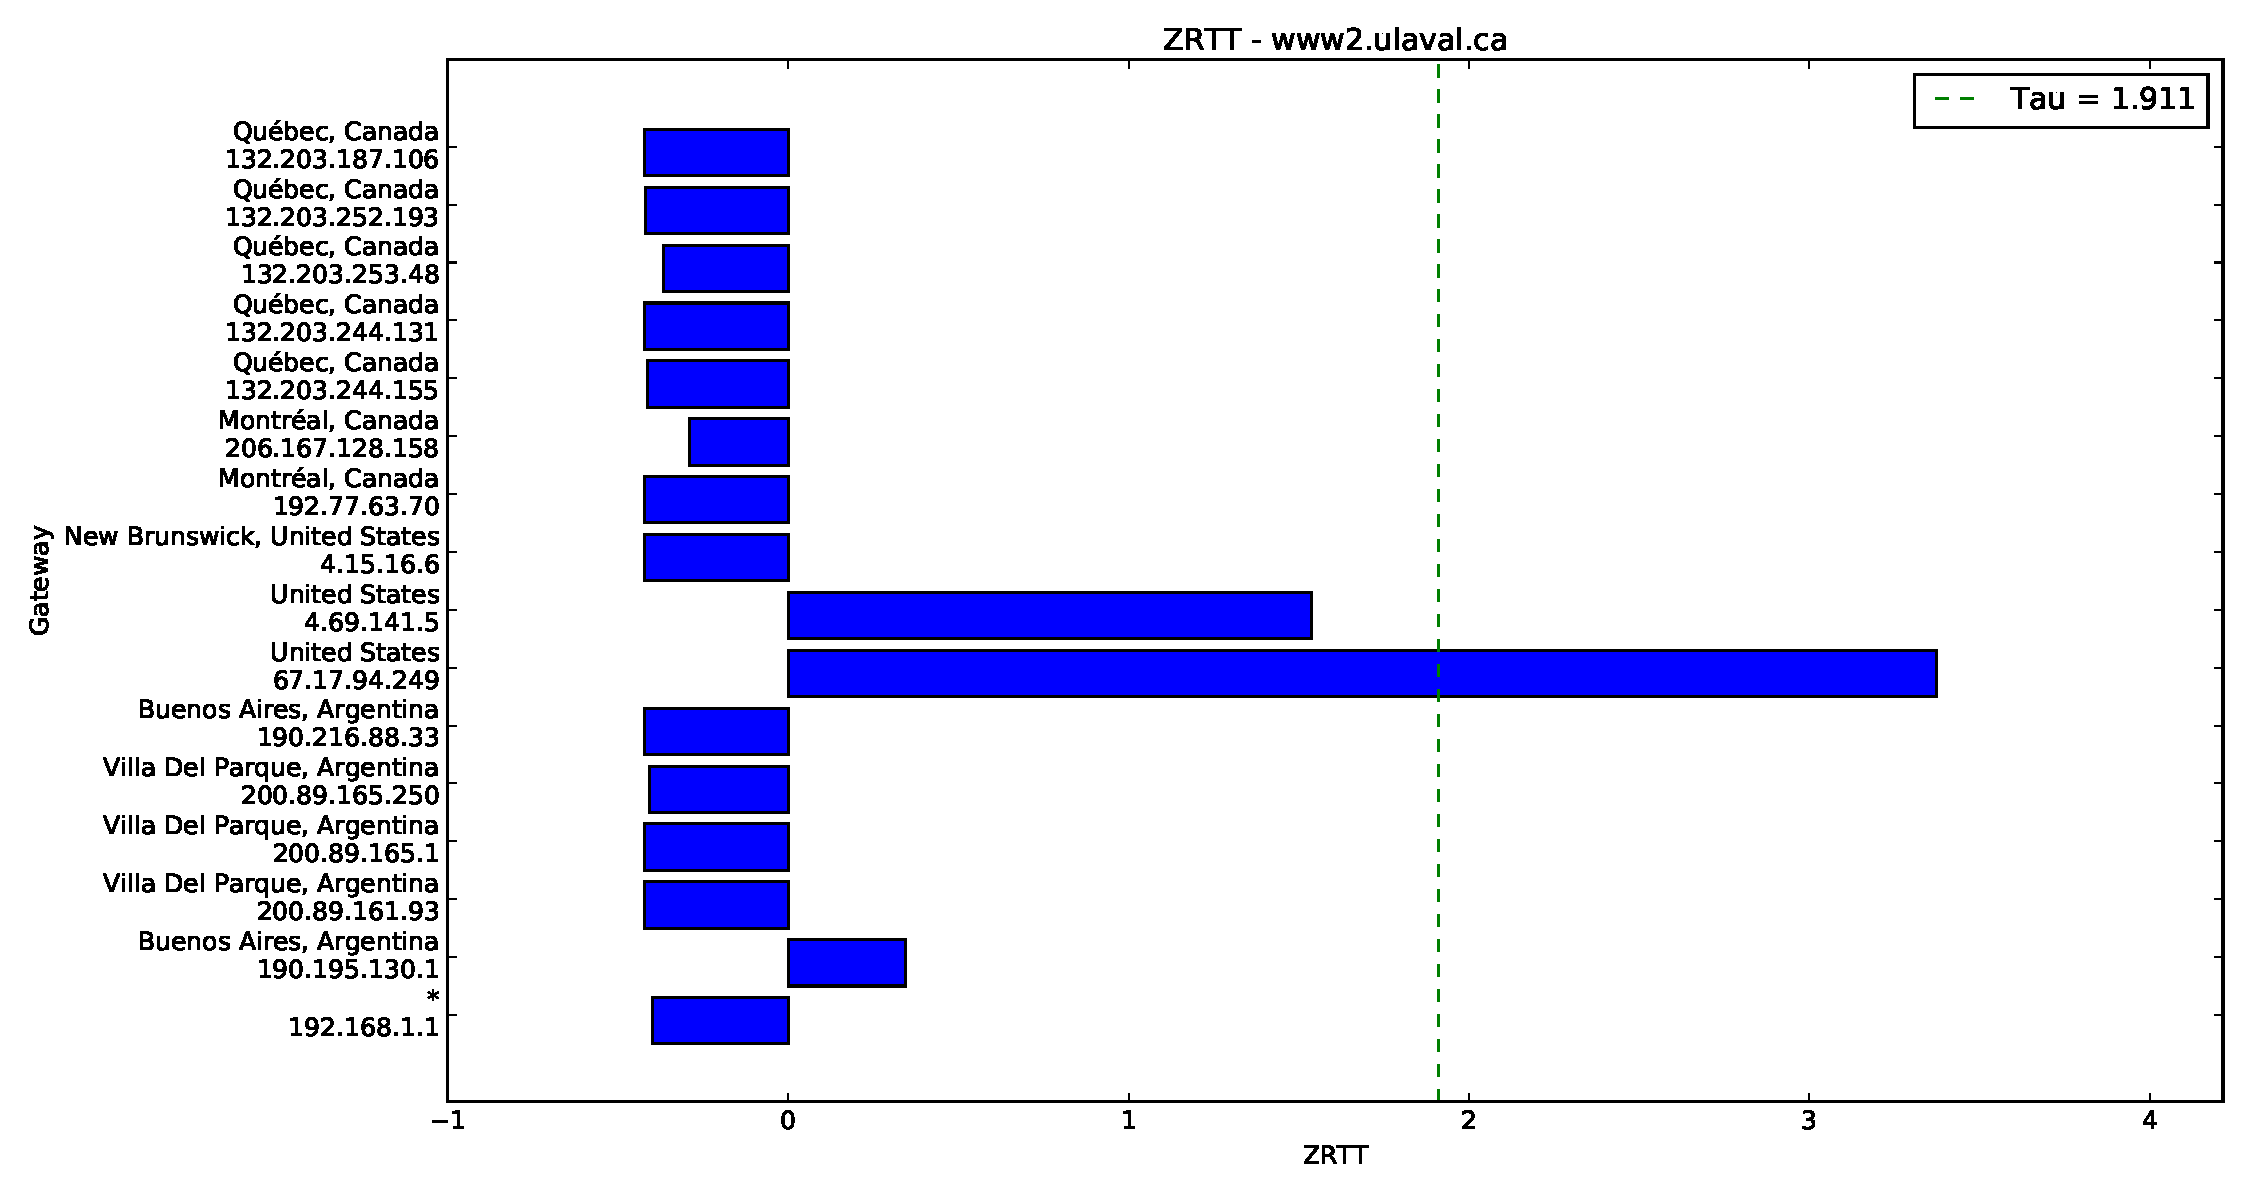
\includegraphics[width=8.5cm]{img/grafico2-www2-ulaval-ca.pdf}
    \caption{\normalfont ZRTTs entre saltos.}
\end{figure}

\begin{figure}[H]
    \centering
    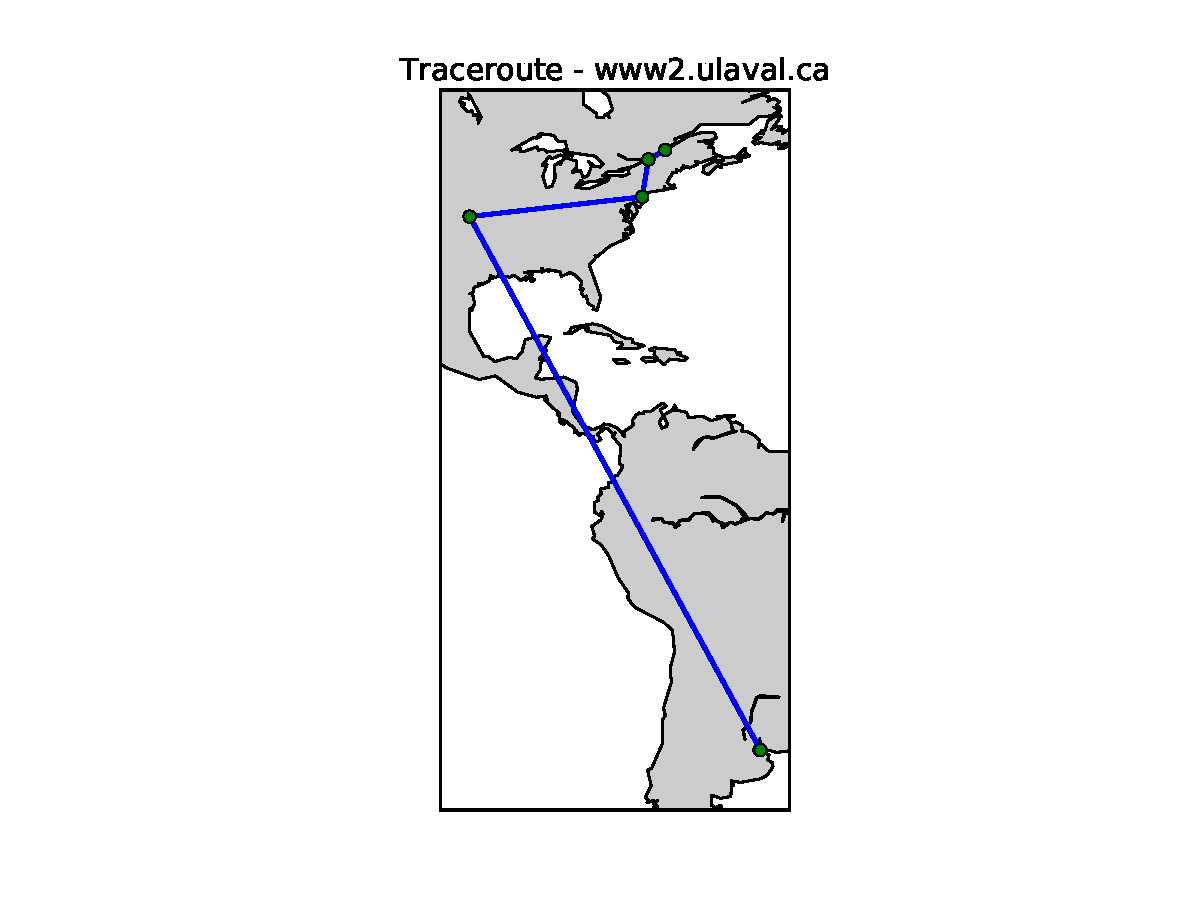
\includegraphics[width=8.5cm]{img/grafico3-www2-ulaval-ca.pdf}
    \caption{\normalfont Ubicación geográfica estimada de la ruta tomada.}
    \label{mapaLaval}
\end{figure}

\par Sólo un salto (de 200.89.165.250 a 67.17.94.249) se presentó como \textit{outlier} según el método planteado\cite{outliers}.
De acuerdo a la estimación geográfica, este salto se da entre Buenos Aires y Estados Unidos.

\par No hay ningún cable submarino que una directamente a Argentina con Estados Unidos.
Sin embargo se pueden trazar rutas submarinas componiendo distintos cables submarinos entre ambos extremos\footnote{Por ejemplo, el South American Crossing (SAC) une a Argentina con Panamá y el Pan-American Crossing (PAC) a Panamá con Estados Unidos.}.

\par Si bien estos dos hechos parecen contradecirse, Jobst 2012\cite{anomalias} provee una explicación: routers de \textit{MPLS}\footnote{\textit{Multiprotocol Label Switching (MPLS)} es un protocolo empleado para simplificar el \textit{forwarding}.} que no honran el campo \textit{TTL}, y por ende no aparecen en la \textit{traceroute}.
Los cables submarinos manejan un flujo muy alto de paquetes, por lo que es esperable que busquen optimizar la performance; ignorar el campo \textit{TTL} es una forma de logarlo.
Esto resulta en que toda la ruta entre Buenos Aires y Estados Unidos se vea condensada en un único salto.

\par Cabe destacar que la herramienta geógrafica utilizada no pudo proveer la latitud y longitud de la dirección IP 67.17.94.249, por lo que el mapa emplea la próxima dirección ubicable, la 4.69.141.5.
